% !TEX root = ../my-thesis.tex
%
\chapter{AutoML with an Ensemble of Optimizers}
\label{sec:approach}
As outlined in the previous chapter, in theory any optimization approach under a resource budget is limited to a set of problem classes, where it can find a solution that is better than any solution another optimization approach could find for the same problem class, i.e. where the approach is superior.
For an actual use-case, as for instance AutoML, it would be necessary to either have significant domain knowledge or to had conducted a broad empirical evaluation to select the optimizer that have a high chance of performing superior for a newly encountered problem class.
This can be avoided, if during the optimization process a set of optimizers would be evaluated in the context of the presented optimization problem and the most apt one would be applied automatically.\newline
Furthermore, it was argued how a separation of the optimization space into model selection and model configuration spaces by optimization space transformations could be beneficial.
The anticipated advantages are a speed-up at first, because the dimensionality of the input space for an optimizer can be reduced.
Secondly, the best suited optimizer for the model configuration can be selected independently from the constructed pipeline after the model selection.\newline
Although this approach could be generalized to any form of algorithm selection and hyperparameter configuration problem, this thesis focusses on the AutoML use-case and therewith has to address well suited machine learning pipelines as an expected output for a wide variety of datasets as an input.
Thus, the constructed pipelines should be able to be as sophisticated as necessary to suit the complexity of any possible input dataset.
Therewith, the approach has the additional requirement of preventing overly stringent limitations of the pipeline topology such as a fix length or solely linear compositions.\newline
In the following chapter such a method will be presented and applied to the AutoML use-case.
This approach will be explained in the following steps in separate sections:
\begin{enumerate}
    \item A short overview how model selection and configuration spaces can be separated for this approach
    \item The structure of the model selection optimization space and how the optimization will be performed to enable the selection of different optimizers for model configuration out of an embedded optimizer ensemble
    \item The structure of the model configuration optimization space and which benefits can be utilized from using and re-using the different optimizers of the ensemble
\end{enumerate}

\section{Separation of Model Selection and Configuration}
\label{sec:approach:separation}
A usual AutoML optimization search space is a joint space for model selection and model configuration consisting out of a set of components, which can be used to construct a machine learning pipeline, and based on the selected components, a valid configuration has to be created.
Since in the joint optimization space the selected components are not known beforehand, the dimensionality of this space has to be selected for a fix parametrization size.
Hence, the model configuration can only create parameter configurations with a pre-defined size as a constraint and the set of pipeline components for model selection can only contain components whose configuration does not exceed this size.\newline
If the model selection and the model configuration steps are performed sequentially on separated optimization spaces, the dimensionality of the model configuration space can depend on the outcome of the model selection step and have the necessary dimensionality for the constructed pipelines parametrization.\newline
Similar to ReinBo and Mosaic, the model selection space is represented by a tree structure.
After the optimization method reaches a leaf node and has therewith complete and valid pipeline structure, the size of the required configuration becomes clear.
Any leaf node is for this reason the connection point and foundation for a model configuration space and the configuration requirements can be deduced.
Thus, dimensionality and structure of the optimization space for the model configuration can be determined from the configuration requirements of the pipeline represented in this leaf node.

\section{Model Selection with MCTS}
\label{sec:approach:selection}
While the overall goal of the model selection step is to construct a pipeline out of a set of pipeline components, in this approach two additional sub-goals come in addition as supplementary requirements:
\begin{enumerate}
    \item The constructed pipeline should be able to be constructed more flexible and more sophisticated than in ReinBo and Mosaic, i.e. have an unrestricted length and no constraints regarding linearity.
    \item The model selection step should be able to evaluate the different optimization methods and their performance regarding the input dataset or even regarding the model configuration for specific pipeline components in the context in the dataset.
    With such an approach, the the most suitable optimizer can be detected and exploited, which will be the key concept for creating an optimizer ensemble.
\end{enumerate}
In the following, both sub-goals will be addressed.
The next two sub-sections tackle the first sub-goal by modelling the model selection process as a graph search problem as first and describing this search graph in more detail afterwards.
Thereafter, in the third sub-section a formalization of the ensemble concept for multiple optimizers is given in the form of a Multi-Armed Bandit problem.
Finally, in the fourth sub-section it is illustrated how both sub-goals can be achieved during the model selection by performing a MCTS.

\subsection{Model Selection as a Graph Search Problem}
\label{sec:appraoch:selection:search}
A machine learning pipeline can vary heavily in structure and complexity.
For example, simple using a Decision tree as the only component as well as many components in a more sophisticated topology as in figure~\ref{fig:appraoch:complex-pipeline} are valid pipelines and depending on the concrete input dataset, both variants could be the optimal output of the model selection step.
\begin{figure}[ht!]
    \centering
    % TODO: Replace figure
    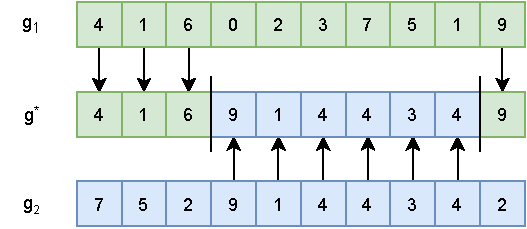
\includegraphics[width=\textwidth]{gfx/Figures/Theory/Crossover.pdf}
    \caption{An example of a complex machine learning pipeline with a higher length and a non-linear topology.}
    \label{fig:appraoch:complex-pipeline}
\end{figure}
Since ReinBo and Mosaic solve their model selection tasks by defining a fix pipeline length and creating a model selection tree containing every combinatorial possible combination from a few different component types, these approaches do not allow complex pipelines.\newline
Other approaches, as for example ML-Plan, TPOT or RECIPE utilize hierarchical task network planning(\textit{HTN planning}) combined with a best-first search or expression trees and formal grammars together with genetic programming, to achieve a more unconstrained model selection optimization space.
Because for the ensemble method a MCTS will be required(will be reasoned in~\ref{sec:appraoch:selection:mcts}), which is a heuristic search algorithm like the best-first search as in ML-Plan, this approach will take this HTN planning approach as a foundation to construct the model selection space.

\subsection{Description of the Search Space Graph}
\label{sec:appraoch:selection:graph}

\Blindtext

\subsection{Multiple Optimization Algorithms as a Multi-Armed Bandit Problem}
\label{sec:appraoch:selection:bandit}

\Blindtext

\subsection{Ensemble Interaction with a MCTS}
\label{sec:appraoch:selection:mcts}

\Blindtext

\section{Model Configuration with Multiple Optimizers}
\label{sec:approach:configuration}

\Blindtext

\subsection{Shared Parameter Domain for Selected Models}
\label{sec:appraoch:configuration:parameter}

\Blindtext

\subsection{Warmstarting Versions of Optimization Algorithms}
\label{sec:appraoch:configuration:warmstart}

\Blindtext